%%% The main file. It contains definitions of basic parameters and includes all other parts.

%% Settings for single-side (simplex) printing
% Margins: left 40mm, right 25mm, top and bottom 25mm
% (but beware, LaTeX adds 1in implicitly)
\documentclass[12pt,a4paper]{report}
\setlength\textwidth{145mm}
\setlength\textheight{247mm}
\setlength\oddsidemargin{15mm}
\setlength\evensidemargin{15mm}
\setlength\topmargin{0mm}
\setlength\headsep{0mm}
\setlength\headheight{0mm}
% \openright makes the following text appear on a right-hand page
\let\openright=\clearpage

%% Settings for two-sided (duplex) printing
% \documentclass[12pt,a4paper,twoside,openright]{report}
% \setlength\textwidth{145mm}
% \setlength\textheight{247mm}
% \setlength\oddsidemargin{14.2mm}
% \setlength\evensidemargin{0mm}
% \setlength\topmargin{0mm}
% \setlength\headsep{0mm}
% \setlength\headheight{0mm}
% \let\openright=\cleardoublepage

%% Generate PDF/A-2u
\usepackage[a-2u]{pdfx}

%% Character encoding: usually latin2, cp1250 or utf8:
\usepackage[utf8]{inputenc}

%% Prefer Latin Modern fonts
\usepackage{lmodern}

%% Further useful packages (included in most LaTeX distributions)
\usepackage{amsmath}        % extensions for typesetting of math
\usepackage{amsfonts}       % math fonts
\usepackage{amsthm}         % theorems, definitions, etc.
\usepackage{bbding}         % various symbols (squares, asterisks, scissors, ...)
\usepackage{bm}             % boldface symbols (\bm)
\usepackage{graphicx}       % embedding of pictures
\usepackage{fancyvrb}       % improved verbatim environment
\usepackage{natbib}         % citation style AUTHOR (YEAR), or AUTHOR [NUMBER]
\usepackage[nottoc]{tocbibind} % makes sure that bibliography and the lists
			    % of figures/tables are included in the table
			    % of contents
\usepackage{dcolumn}        % improved alignment of table columns
\usepackage{booktabs}       % improved horizontal lines in tables
\usepackage{paralist}       % improved enumerate and itemize
\usepackage{xcolor}         % typesetting in color

%%% Basic information on the thesis

% Thesis title in English (exactly as in the formal assignment)
\def\ThesisTitle{Automatic generation of medical reports from chest X-rays}

% Author of the thesis
\def\ThesisAuthor{Bc. Lukáš Chaloupský}

% Year when the thesis is submitted
\def\YearSubmitted{2022}

% Name of the department or institute, where the work was officially assigned
% (according to the Organizational Structure of MFF UK in English,
% or a full name of a department outside MFF)
\def\Department{Institute of Formal and Applied Linguistics}

% Is it a department (katedra), or an institute (ústav)?
\def\DeptType{Institute}

% Thesis supervisor: name, surname and titles
\def\Supervisor{Mgr. Rudolf Rosa, Ph.D.}

% Supervisor's department (again according to Organizational structure of MFF)
\def\SupervisorsDepartment{Institute of Formal and Applied Linguistics}

% Study programme and specialization
\def\StudyProgramme{Computer Science}
\def\StudyBranch{Software and Data Engineering}

% An optional dedication: you can thank whomever you wish (your supervisor,
% consultant, a person who lent the software, etc.)
\def\Dedication{%
First of all, I would like to thank my supervisor Mgr. Rudolf Rosa, Ph.D. for all his time, guidance and valuable advices he gave me while working on this thesis. I would also like to thank my parents for their unlimited support and patience during my studies.
}

% Abstract (recommended length around 80-200 words; this is not a copy of your thesis assignment!)
\def\Abstract{%
This thesis deals with the problem of automatic generation of medical reports in the Czech langugage based on the input chest X-ray images using deep neural networks. The first part deals with the analysis of problem itself including comparison of existing solutions from several common points of view. In order to interpret medical images in the Czech language we present a fine-tuned a Czech GPT2 model specialized on medical texts based on the original pre-trained English GPT2 model along with its evaluation. In the second part the created Czech GPT2 is used for training neural network model for generating medical reports. The training was conducted on freely available data along with data pre-processing and their adjustment for the Czech language. Furthermore the model results are discussed and evaluated using standard metrics for natural language processing to determine the performance.
}

% 3 to 5 keywords (recommended), each enclosed in curly braces
\def\Keywords{%
{natural language processing}, {image captioning}, {x-ray}, {medical report generation}
}

%% The hyperref package for clickable links in PDF and also for storing
%% metadata to PDF (including the table of contents).
%% Most settings are pre-set by the pdfx package.
\hypersetup{unicode}
\hypersetup{breaklinks=true}

% Definitions of macros (see description inside)
%%% This file contains definitions of various useful macros and environments %%%
%%% Please add more macros here instead of cluttering other files with them. %%%

%%% Minor tweaks of style

% These macros employ a little dirty trick to convince LaTeX to typeset
% chapter headings sanely, without lots of empty space above them.
% Feel free to ignore.
\makeatletter
\def\@makechapterhead#1{
  {\parindent \z@ \raggedright \normalfont
   \Huge\bfseries \thechapter. #1
   \par\nobreak
   \vskip 20\p@
}}
\def\@makeschapterhead#1{
  {\parindent \z@ \raggedright \normalfont
   \Huge\bfseries #1
   \par\nobreak
   \vskip 20\p@
}}
\makeatother

% This macro defines a chapter, which is not numbered, but is included
% in the table of contents.
\def\chapwithtoc#1{
\chapter*{#1}
\addcontentsline{toc}{chapter}{#1}
}

% Draw black "slugs" whenever a line overflows, so that we can spot it easily.
\overfullrule=1mm

%%% Macros for definitions, theorems, claims, examples, ... (requires amsthm package)

\theoremstyle{plain}
\newtheorem{thm}{Theorem}
\newtheorem{lemma}[thm]{Lemma}
\newtheorem{claim}[thm]{Claim}

\theoremstyle{plain}
\newtheorem{defn}{Definition}

\theoremstyle{remark}
\newtheorem*{cor}{Corollary}
\newtheorem*{rem}{Remark}
\newtheorem*{example}{Example}

%%% An environment for proofs

\newenvironment{myproof}{
  \par\medskip\noindent
  \textit{Proof}.
}{
\newline
\rightline{$\qedsymbol$}
}

%%% An environment for typesetting of program code and input/output
%%% of programs. (Requires the fancyvrb package -- fancy verbatim.)

\DefineVerbatimEnvironment{code}{Verbatim}{fontsize=\small, frame=single}

%%% The field of all real and natural numbers
\newcommand{\R}{\mathbb{R}}
\newcommand{\N}{\mathbb{N}}

%%% Useful operators for statistics and probability
\DeclareMathOperator{\pr}{\textsf{P}}
\DeclareMathOperator{\E}{\textsf{E}\,}
\DeclareMathOperator{\var}{\textrm{var}}
\DeclareMathOperator{\sd}{\textrm{sd}}

%%% Transposition of a vector/matrix
\newcommand{\T}[1]{#1^\top}

%%% Various math goodies
\newcommand{\goto}{\rightarrow}
\newcommand{\gotop}{\stackrel{P}{\longrightarrow}}
\newcommand{\maon}[1]{o(n^{#1})}
\newcommand{\abs}[1]{\left|{#1}\right|}
\newcommand{\dint}{\int_0^\tau\!\!\int_0^\tau}
\newcommand{\isqr}[1]{\frac{1}{\sqrt{#1}}}

%%% Various table goodies
\newcommand{\pulrad}[1]{\raisebox{1.5ex}[0pt]{#1}}
\newcommand{\mc}[1]{\multicolumn{1}{c}{#1}}


% Title page and various mandatory informational pages
\begin{document}
%%% Title page of the thesis and other mandatory pages

%%% Title page of the thesis

\pagestyle{empty}
\hypersetup{pageanchor=false}
\begin{center}

\centerline{\mbox{
\includegraphics[width=166mm]{../img/logo-en.pdf}}}

\vspace{-8mm}
\vfill

{\bf\Large MASTER THESIS}

\vfill

{\LARGE\ThesisAuthor}

\vspace{15mm}

{\LARGE\bfseries\ThesisTitle}

\vfill

\Department

\vfill

{
\centerline{\vbox{\halign{\hbox to 0.45\hsize{\hfil #}&\hskip 0.5em\parbox[t]{0.45\hsize}{\raggedright #}\cr
Supervisor of the master thesis:&\Supervisor \cr
\noalign{\vspace{2mm}}
Study programme:&\StudyProgramme \cr
\noalign{\vspace{2mm}}
Study branch:&\StudyBranch \cr
}}}}

\vfill

% Zde doplňte rok
Prague \YearSubmitted

\end{center}

\newpage

%%% Here should be a bound sheet included -- a signed copy of the "master
%%% thesis assignment". This assignment is NOT a part of the electronic
%%% version of the thesis. DO NOT SCAN.

%%% A page with a solemn declaration to the master thesis

\openright
\hypersetup{pageanchor=true}
\pagestyle{plain}
\pagenumbering{roman}
\vglue 0pt plus 1fill

\noindent
I declare that I carried out this master thesis independently, and only with the cited
sources, literature and other professional sources. It has not been used to obtain another
or the same degree.

\medskip\noindent
I understand that my work relates to the rights and obligations under the Act No.~121/2000 Sb.,
the Copyright Act, as amended, in particular the fact that the Charles
University has the right to conclude a license agreement on the use of this
work as a school work pursuant to Section 60 subsection 1 of the Copyright~Act.

\vspace{10mm}

\hbox{\hbox to 0.5\hsize{%
In \hbox to 6em{\dotfill} date \hbox to 6em{\dotfill}
\hss}\hbox to 0.5\hsize{\dotfill\quad}}
\smallskip
\hbox{\hbox to 0.5\hsize{}\hbox to 0.5\hsize{\hfil Author's signature\hfil}}

\vspace{20mm}
\newpage

%%% Dedication

\openright

\noindent
\Dedication

\newpage

%%% Mandatory information page of the thesis

\openright

\vbox to 0.5\vsize{
\setlength\parindent{0mm}
\setlength\parskip{5mm}

Title:
\ThesisTitle

Author:
\ThesisAuthor

\DeptType:
\Department

Supervisor:
\Supervisor, \SupervisorsDepartment

Abstract:
\Abstract

Keywords:
\Keywords

\vss}

\newpage

\openright
\pagestyle{plain}
\pagenumbering{arabic}
\setcounter{page}{1}


%%% A page with automatically generated table of contents of the master thesis

\tableofcontents

%%% Each chapter is kept in a separate file
\chapter*{Introduction}
\addcontentsline{toc}{chapter}{Introduction}

In hospital, inspecting the X-rays and writing corresponding medical reports is a hard work that requires experienced specialized doctors, of which there are not many. A great deal of people visit hospitals daily and X-rays are taken for many of them. Automatic interpretation of X-ray image has a great potential to improve health care and it could be particulary helpful to doctors in order to distinguish serious cases from the ordinary ones and overall accelerate and improve their work.\\

Automatic generation of radiology reports is a subset of a general problem called Image Captioning, i.e. generation of overall textual captions to input images. Image captioning is a combination of Natural Language Processing and Computer Vision areas, experiencing a lot of progress in the last years. Most often the Image Captioning problem is solved using Deep Learning techniques. The specificity of this subset is that we do not want to generate just a general caption of the image, but the exact description of all findings contained in the given medical image. There were done multiple studies for this task in other languages but none in the Czech language.\\

Deep learning by its very nature has wide range of uses in a medical sector as it can often capture complex relations in any kind of data with excellent performance results. Nevertheless, in the medical environment the accuracy of predictions is crucial in order to determine the final diagnosis. Therefore, we should not consider the models as such as something that is unmistakably true, but as an auxiliary tool that should help doctors to examine X-rays.\\

Inasmuch as it is not so challenging to detect fractures on the limbs, this area is less interesting than others which have a variety of diverse possible problems. One of these areas is chest for which there exists multiple freely accessible datasets containing full textual medical reports. However, all these available datasets have one common downside, they are not in the Czech language. The natural question arises, where do we obtain these much needed data? We have to face and solve this core problem in our thesis.\\

\section*{Goals}
First of all, we will take a closer look at the problem itself. This includes breaking down the problem and analyzing all its parts individually together with presenting possible existing alternatives for each part. \\

The main target of our thesis is to train a neural network for the purpose of generating textual medical reports for X-ray images. An example of our problem can be seen in Figure \hyperref[fig01:ProblemExample]{1.1} for illustration.\\
\newpage

Our first goal is to fine-tune a language model directly for the Czech language. The language model will be specialized directly to medical texts in order to capture the essence of the problem. However, ahead of the medical specialization, we want to fine-tune a general Czech language model. Fine-tuning will be based on the original English GPT-2 model presented in \citet{radford2019language}.\\

Finally, we want to utilize our fine-tuned language model for training a neural network model interpreting chest X-rays images and generating corresponding medical textual reports to them in the Czech language. This section also involves the overall data preparation directly for the Czech language. In addition, the training will be done in multiple setups. All possibilities will be evaluated with the purpose of determination of their final performance.\\

\section*{Thesis structure}

In the very first chapter we present a detailed description of our problem. Every aspect of our problem is introduced and all existing solutions or possibilities are discussed with their pros and cons. Moreover we introduce there some of the important related works.\\

Following chapter is dealing with the design of solution to our problem, with all reasonings and decisions made. This includes not only the final neural network model, but also the language model fine-tuning and data preparation.\\

Technical details about the implemented scripts are described in the third chapter.\\

All experiments done with our models take their part in the fourth chapter, describing all used environments and differents setups together with data variants. This section also contains partial results of the GPT-2 training.\\

Whole fifth chapter is then dedicated to evaluation of experiments done in the preceding part. Furthermore, our models will be compared to the performance of other existing solutions.\\

Finally, in epilog we discuss what we have accomplished in the thesis, what the resulting consenquences are and what the future possibilities are.
\chapter{Problem Analysis}
This chapter deals with the overall analysis of the problem itself. In the very beginning we present the definition of the problem. Every aspect of the problem is further discussed in detail along with a comparison of possible solutions. Moreover, the next section of the chapter describes data we work with and their alternatives. The final part of this chapter presents some of the important related works.

\section{Methods of generation}
\label{sec:methodsOfGeneration}
First of all, we will present posssible approaches for image caption generation. Inasmuch as almost all solutions for image captioning based on neural networks are using an encoder-decoder architecture as their core with further minor or major adjustments we will discuss just this architecture. Encoder serves for the purposes of extracting visual features from the input images into intermmediate vector representations for the decoder. The decoder is subsequently fed with these visual feature vectors and decodes them token by token into the natural language text.\\

Moreover, over the past years the encoder-decoder architecute has been enhanced using the attention mechanism. The problem of encoder-decoder architecture without any other mechanism is that all the information about the image have to be encoded globally inside a single vector. However not all the information about the image is relevant for the caption generation. For this reason the attention mechanism was introduced. Instead of a single vector, the set of feature vectors representing the spatial information of the input image is used. This allows us to dynamically focus only on specific areas during the generation. The overall nature of the mechanism is derived from the way our brains concentrace on the images.\\

Attention mechanism for image captioning was first introduced in the \citet{xu2015show} work using the Bahdanau attention proposed in \citet{bahdanau2014neural}. After extractions of visual feature vectors $h_j$ from image, we want to assign a weight $\alpha_{ij}$ to each of this vectors indicating the relevance of the image position $j$ when generating output at position $i$. This results in the context vector $c_i$, a dynamic weigthed combination of $h_j$ features, that is presented as another input to the decoder. All attention calculations are defined as follows:
\begin{equation}\label{eq01:AttContext}
	c_i = \sum_{j=1}^{t} \alpha_{ij} h_j
\end{equation}

\begin{equation}\label{eq01:AttWeights}
	\alpha_{ij} = \frac{\exp(e_{ij})}{\sum_{k=1}^{t} \exp(e_{ik})}
\end{equation}

\begin{equation}\label{eq01:AttFeedForwardNetwork}
	e_{ij} = a(s_{i-1}, h_j)
\end{equation}

where $s_{i-1}$ is a previous hidden state and $a(s_{i-1}, h_j)$ is an attention model.

\subsection{Encoder}
Encoder is responsible for extracting high-level visual features of the input image into one or more visual feature vectors. Moreover, the encoder can include also additional parts for another independent purposes, e.g. detection of objects in the image and their classification, which may be further passed to the decoder as a separate or an extra input. We will describe some of the most used neural network architectures utilized as an encoder.

\subsubsection{Convolutional neural networks}
Convolutional neural networks (CNN)\footnote[1]{\url{https://en.wikipedia.org/wiki/Convolutional\_neural\_network}} are the most leveraged type of neural networks for the purposes of image analysis. They are applying 2D convolution filters for all positions in the image with the shared weights allowing to detect similar patterns independently on the position. Each layer of filters will downsize the dimensions of the previous layer and increases the number of filters. By gradually applying filters, the network is learning more complex patterns.\\

Instead of training convolutional neural networks from scratch, already pretrained CNN models are often used and possiblly further fine-tuned to a specific area. These models have been trained on a vast amount of data thanks to which they learned to recognize a relevant features in the lower layers applicable to any kind of images. In contrast, training from scratch is costly and takes a much longer time. Among the used pre-trained CNN model architectures are for example ResNet\citep{he2016deep}, VGGnet\citep{simonyan2014very}, DenseNet\citep{huang2017densely} or EfficientNet\citep{tan2019efficientnet}.

\subsubsection{Transformers}
\label{sec:transformersEncoder}
With the \citet{vaswani2017attention}, a new neural network archtecture called tranformers was introduced. The transformers are using multi-head self-attention mechanism to compute the relations between the elements in the sequences. Although the transformers were originally designated for NLP tasks, they can be also utilized for other domains like images due to their robustness. Vision transformers (ViT), presented in \citet{dosovitskiy2020image}, is an adaptation of transformers encoder for image classification without any CNNs. The core of the encoder is identical to the one in the original transformer. Nevertheless, the input image is represented as a sequence of patches for which their embeddings are computed together with the positional encodings as the input, as we can see in the Figure \hyperref[fig01:ViT]{1.1}.

\begin{figure}[h]\centering
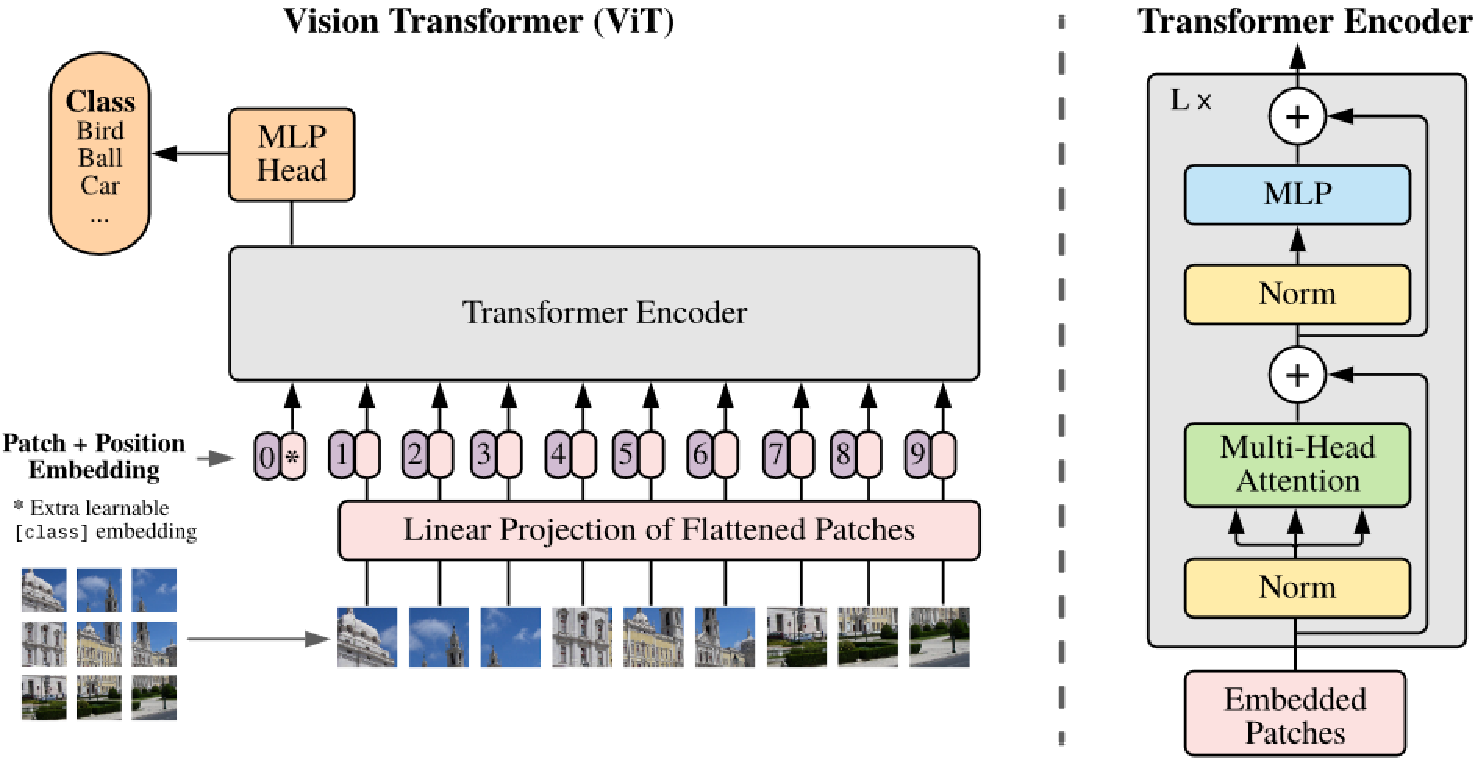
\includegraphics[width=145mm, height=76mm]{../img/VisualTransformerArchitecture}
\caption{Visual Transformer architecture from \citet{dosovitskiy2020image}.}
\label{fig01:ViT}
\end{figure}

\subsection{Decoder}
The second main part of the network is the decoder which serves as a language model for generating corresponding captions to input images. During the generation process the visual features of the image from the encoder and the already generated text are taken into account for the predtiction of the next token or word. In the process of generation, the attention mechanism (described above in the Chapter \ref{sec:methodsOfGeneration}) is almost always incorporated in order to focus only on the substantial particular areas. The following subsections presents common approaches used as the backbones for the decoder part of the network.
\subsubsection{Recurrent neural networks}
Recurrent neural networks (RNN)\footnote[2]{\url{https://en.wikipedia.org/wiki/Recurrent\_neural\_network}} are a category of neural networks designated for sequence data processing. Context of the previous part of the sequence can influnence the subsequent elements due to the RNN cell's internal memory (hidden state). Each time step RNN cell computes its activation function from current input and hidden state producing updated hidden state as output. For language modeling tasks, the last generated token or word is given to the RNN as the next input until the entire text is produced. The autoregressiveness of the RNNs is the reason why they are ideal for use as a language model. The two most used types of RNN cells are LSTM\citep{hochreiter1997long} and GRU\citep{cho2014learning}, however the LSTM cells are more utilized as the decoder because they can remember longer sequences. Moreover, we can combine them in a hierarchical manner to capture more complex structures in the generated text. Neverthless, the downside of the RNNs is the training time due to their sequential nature. The whole sentence must pass through RNN token by token and cannot be parallelized.

\subsubsection{GPT2}
Just as in the case of encoder, with the advent of transformers presented in the \citet{vaswani2017attention} paper, the deoder part of transformers started to be used as the language model for image captioning task for their great results in the natural language processing (NLP)\footnote[3]{\url{https://en.wikipedia.org/wiki/Natural\_language\_processing}} tasks. One of the advantages of the transformers against the previously used recurrent neural networks is the loss of the need for sequential processing during the training. Due to the fact that the processing of the whole caption can be done in parallel, the entire training process is significatnly accelerated. Moreover, the transformers can capture longer ranges dependencies in the text, as they process the sentence as a whole instead of sequentially by words.\\

One of the state-of-the-art autoregressive language models using transformers as their backbone is OpenAI GPT-2 model from the \citet{radford2019language} paper, which outperforms other language models on many NLP tasks. It was trained on a massive English dataset called WebText (introduced in the same article) containing a total of 40 GB of raw text. The resuling model is able to generate large coherent texts. Furthermore, it can be fine-tuned to a different domain or to a completely different language.

\section{Data}
In previous part we talked about possible methods of generation. Another crucial aspect we need to discuss are data, which are a basic building block of our thesis. This part focuses on the analysis of the data we used in our thesis, but also on their alternatives. \\

In order to solve our task and train neural network we need to get dataset containing the X-rays images along with their textual descriptions and optionally some other attributes of the examined X-rays. Moreover, the fundamental feature we need is that the data must be in the Czech language.

\subsection{Existing datasets}
\label{sec:datasets}
Medical environment provides a plenty of diverse potential problems, which can be researched. As already mentioned, in this thesis we focus specifically on the X-ray images. Because it is not so hard to detect fractures on the limbs, this area is not as interesting as others. One area that is rich in its diversity is the chest. As a result, this area is explored the most and therefore there exists multiple datasets with full textual mecidal reports. In the following section we describe some of them.\\

Apart from the datasets described below, other datasets with similar type are being used with the aim of solving our task. Amongst them belong datasets such as ImageCLEFmed~Caption\citep{ImageCLEFmedicalCaptionOverview2022}, PadChest\citep{bustos2020padchest}, BCIDR\citep{zhang2017mdnet} and PEIR~Gross\citep{jing2017automatic}. Moreover, except for datasets containing textual reports there exist a lot of other datasets worth mentioning containing different kind of information for each X-ray. These include, for example, CheXpert\citep{irvin2019chexpert}, VinDr-CXR\citep{nguyen2020vindr}, ChestX-ray8\citep{wang2017chestx} and its expanded version ChestX-ray14.

\subsubsection{Indiana University chest X-ray}
\label{sec:IUDataset}
Indiana University chest X-Ray dataset has become a standard in the field of medical report generation, it was presented in the \citet{10.1093/jamia/ocv080} paper. This dataset is an open source collection of pairs of chest X-rays and their corresponding semi-stuctured textual radiology reports, which is freely availble on the web\footnote[4]{\url{https://openi.nlm.nih.gov/faq\#collection}} without any additional requirements. We have a choice if we want to download just reports or images and in either PNG or DICOM format. The entire dataset consists of 7470 chest X-ray images that cover not only the frontal (PA\footnote[5]{Posterior-Anterior}) view, but also the lateral (side) one. These images corresponds to a total of 3995 patient's medical text reports.\\

Figure \hyperref[fig01:IUChestXRaySample]{1.1} shows an example from the Indiana University chest X-ray dataset. Each dataset pair is carefully de-identified in order to remove any personal information. The text of the report is semi-structured in up to 5 sections. The most important sections are \textit{impression}, where the overall diagnosis is stated, \textit{findings} section describing the details of examination and \textit{tags} which are of two types - manual and automatic. Manual tags were annotated manually using MeSH\footnote[6]{\url{https://www.nlm.nih.gov/mesh/meshhome.html}} and RadLex\footnote[7]{\url{http://radlex.org/}} codes, automatic were encoded from the reports using the MTI indexer. The rest of the sections are \textit{indication} and \textit{comparison}.\\

The disadvantage of this dataset is that it is relatively small. On the other hand, it is a clean and manually checked dataset containing also additional information about images in a form of tags described above.

\begin{figure}[h]\centering
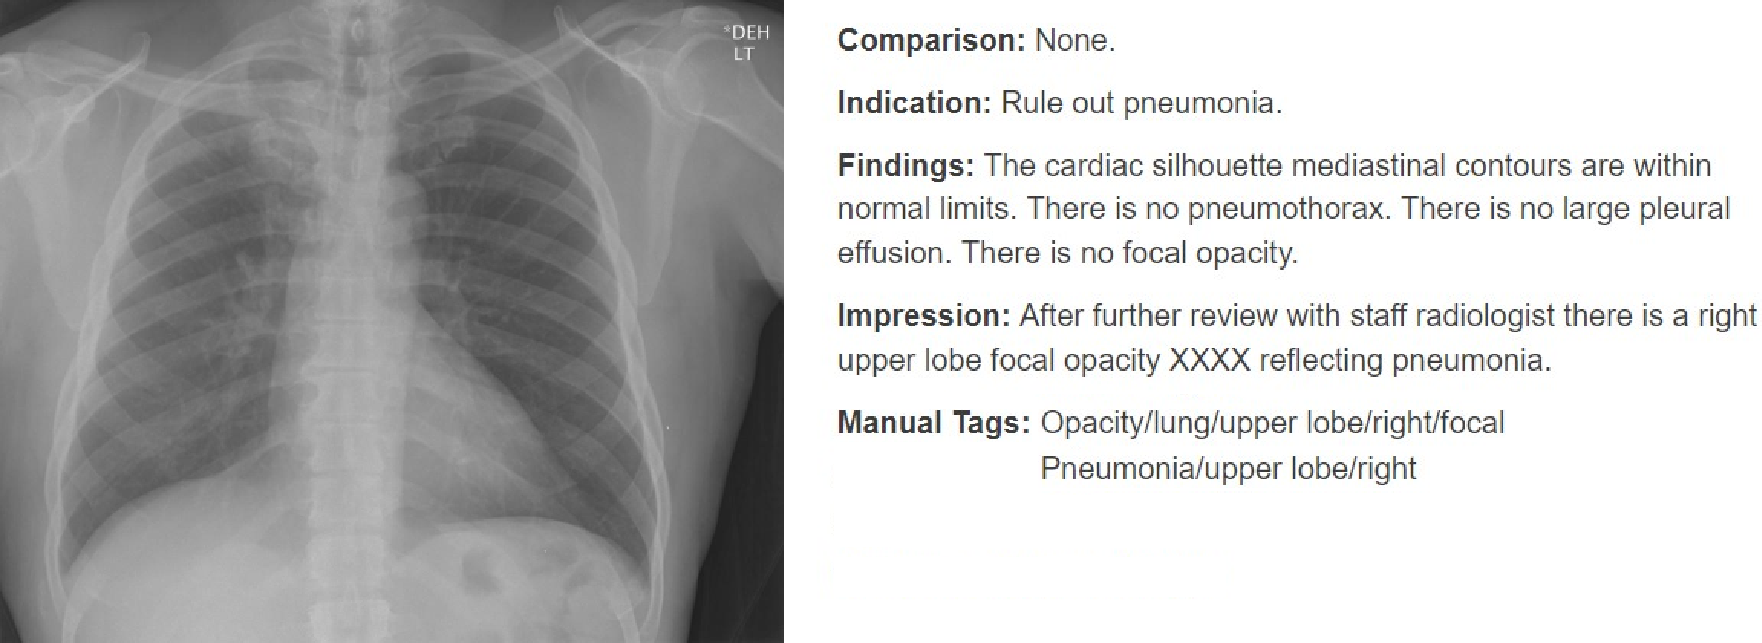
\includegraphics[width=145mm, height=53mm]{../img/IUChestXRaySample_CXR1728_IM-0479-1001}
\caption{Sample from the Indiana University Chest X-ray dataset.}
\label{fig01:IUChestXRaySample}
\end{figure}

\subsubsection{MIMIC-CXR v2.0.0}
MIMIC-CXR v2.0.0 is another dataset consisting of full semi-structured medical textual reports against corresponding chest X-rays that was presented in the \citet{cxr:johnson2019mimic} paper. As the previous dataset, it is openly available on the web\footnote[8]{\url{https://physionet.org/content/mimic-cxr/2.0.0/}}. In order to get access to the dataset, we have to go through registration and verification steps. The verification phase includes completion of CITI\footnote[9]{\url{https://about.citiprogram.org/series/human-subjects-research-hsr/}} \textit{Data or Specimens Only Research} course for \textit{Human Subject Research}. Moreover we need somebody trustworthy as a reference to confirm the authenticity of our identity. After the verification we get access to all datasets in the same repository.\\

The dataset consists of 377,110 X-ray images in the DICOM\footnote[10]{\url{https://www.dicomstandard.org/}} format connected to a total of 227,835 radiology reports for 65,379 patients. Each report is structured into multiple different sections. In order to satisfy legal requirements, entire dataset is automatically de-identified to remove any protected~health~information\footnote[11]{\url{https://en.wikipedia.org/wiki/Protected\_health\_information}}. Similalry to the previous dataset the essential two sections of each report are \textit{impression} and \textit{findings}. There also exists older MIMIC-CXR-JPG\footnote[12]{\url{https://physionet.org/content/mimic-cxr-jpg/2.0.0/}} dataset, presented in the \citet{cxr-jpg:johnson2019mimic} paper. This is an older version of MIMIC-CXR v2.0.0 dataset consisting of the exactly same images, only in JPG format, but each image is assigned 14 labels indicating the presence of the category in the report instead of its textual form. Each category has assigned either a \textit{1}, \textit{0} or \textit{-1} label with the meaning \textit{positively mentioned}, \textit{negatively mentioned} or \textit{uncertain}. The labels were determined from the reports utilizing the CheXpert\citep{irvin2019chexpert} and the NegBio\citep{peng2018negbio} open-source labelers.\\

The advantage of this dataset is its vast number of samples. Moreover, as described above, we can get additional information in a form of categories to every image. Nevertherless the textual reports carry some noise in them in the form of grammatical mistakes and incorrect formatting. We face these issues in the Chapter X. 

\begin{figure}[h]\centering
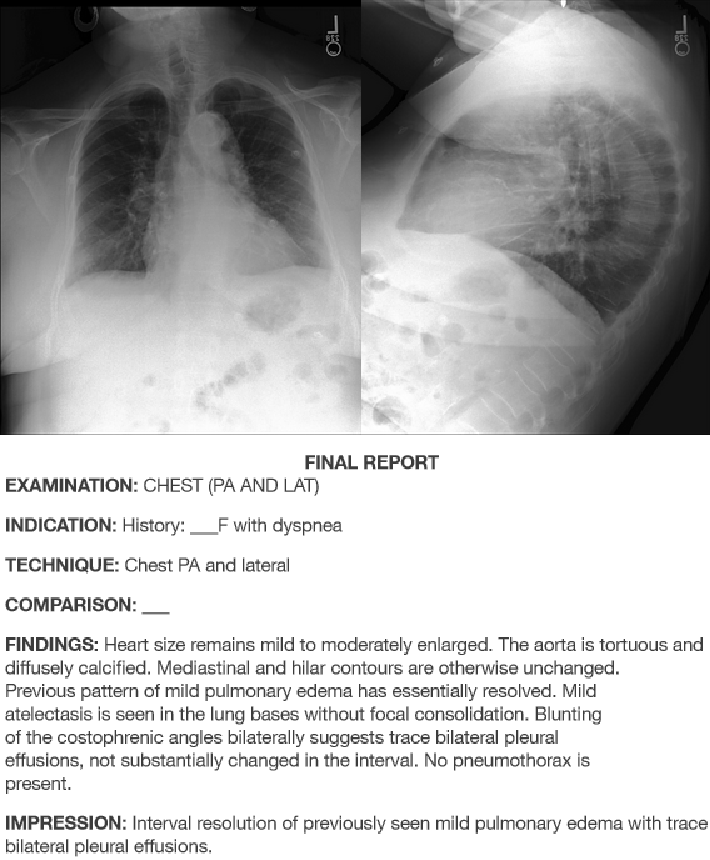
\includegraphics[width=135mm, height=163mm]{../img/mimic_s57861150}
\caption{Sample from the MIMIC-CXR dataset.}
\label{fig02:MimicCXRSample}
\end{figure}

\newpage

\subsection{Czech data}
All freely available datasets presented in the previous part have one common downside, namely they are not in the Czech language. As a part of elaboration of this thesis an intesive communication with real czech hospitals and other possible sources of real data took place. The goal of this communication was to create the very first open czech dataset of this kind. Processing of this kind of data would mean not only preparing the data into suitable format but also it would include proper anonymization of any personal information about the patients within the data. \\

However, inasmuch as the authentic patients data from hospitals are subject to strict privacy rules and we are not employees of any hospital, the institutions decided that they cannot provide the data in any way without the concious permission of patients given before the examination. With this result we need to find a different way how to obtain this much needed czech data.

\subsection{Translators}
In the previous sections we discovered that there is no dataset in the Czech language for our problem and there is no easy way how to get acces to the real data in order to build one. The only thing left is to create a new artificial dataset using an automatic translation. We will compare different freely accesible translators and choose the right one for our needs.

\subsubsection{DeepL}
At the moment, DeepL\footnote[13]{\url{https://www.deepl.com/translator}} translator provides the finest available translations beating even the ones from Google Translate. Moreover, it has freely usable web application and REST API. However, the main drawback of the DeepL translator is that its REST API is highly limited - only 500 000 characters per month can be translated for free. Furthermore, any translation above this limit is costly and thus this path is not appropriate for translating large textual datasets. One way to get around this problem is to use their internal REST API used specifically for the web application, which is free to use. We investigated and implemented this potential way in our thesis and further experimented how much it can be used, but unfortunately even this internal REST API is strictly limited for only tens of consecutive\footnote[14]{REST API calls are delayed from each other for some time, otherwise the service is blocked immediately} translations making it unusable for out needs.

\subsubsection{Google Translate}
Google~Translate\footnote[15]{\url{https://translate.google.com/}} has become already de facto standard in the world of machine translation and it is the most used freely accessible language translation service in the world. In terms of quality, the translations are still great although little bit worse than those from DeepL. The web application is free of any charge and anybody can use it as much as he needs. Nevertheless, just as in the case of DeepL, their REST API services are limited and translation of anything above that limit is expensively charged. For these reasons, as in the previous case, we must find another way.

\subsubsection{CUBBITT}
Machine~Translation\footnote[16]{\url{https://en.wikipedia.org/wiki/Machine\_translation}} is an extensive area of research, as a result of which there exist many other projects and academic papers nowadays. One of them is CUBBITT\footnote[17]{\url{https://lindat.mff.cuni.cz/services/translation/}} translator, which was developed at our faculty. The whole system is presented and described in detail in the \citet{biblio:PoToTransformingmachine2020} paper. \\

CUBBITT translator provides translations which are comparable to the ones from DeepL and Google Translate services. As other mentioned translators it provides an openly available web application for machine translation. Moreover and most importantly it provides REST API that is completely unlimited in text volume and free to use without any additional charges. These are the reasons why we will utilize CUBBITT in our thesis as a translator to create our artificial dataset.\\

On the other hand, CUBBITT has not support for auto-correcting input text compared to above mentioned services. Moreover, there are some patterns in the text which CUBBITT cannot translate at all or translates them incorrectly. These problems complicates our situation as the data from hospitals carry some natural noise in them. We face these complications in Chapter X.

\section{Related work}
\label{sec:RelatedWork}
The last section of this chapter is dedicated to the description and comparison to some of the related works that solves identical or similar problem as we do.\\

The most significant related work is \citet{alfarghaly2021automated} inasmuch as we base our thesis on it. This paper focuses on the identical problem as we do, only in the English language. The proposed solution uses a pre-trained and further fine-tuned Chexnet model, presented in \citet{rajpurkar2017chexnet}, as a visual features encoder and distilGPT2 language model\citep{radford2019language} as a decoder which is additionally conditioned on the visual features and predicted tag's word2vec\citep{mikolov2013distributed} embeddings. For training the neural network the Indiana University chest X-ray dataset, described in more detail in Chapter \ref{sec:IUDataset}, is used. Figure \hyperref[fig03:OmarExample]{1.3} shows examples of the model outputs.\\

\begin{figure}[h]\centering
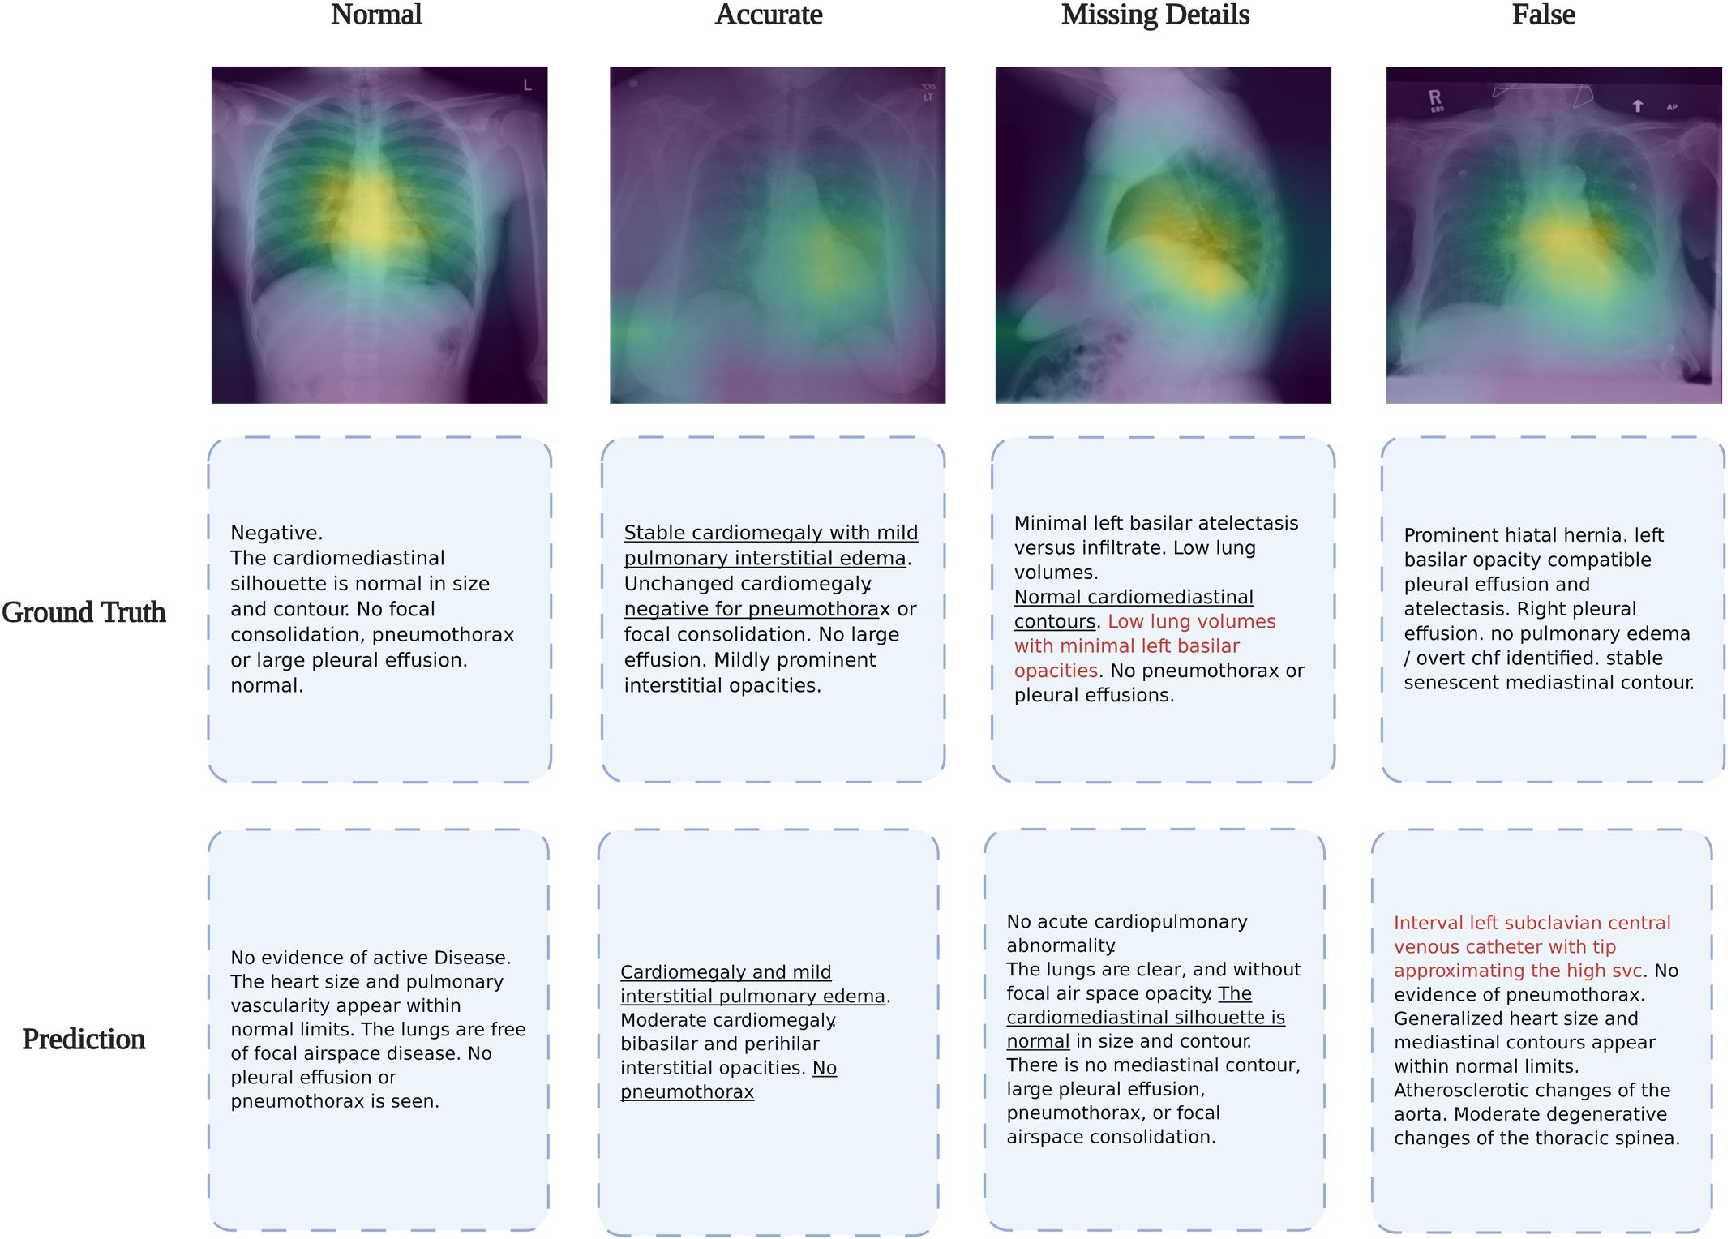
\includegraphics[width=145mm, height=104mm]{../img/OmarExample}
\caption{Examples of generated medical reports from \citet{alfarghaly2021automated}.}
\label{fig03:OmarExample}
\end{figure}

Another paper making use of transformers is \citet{chen2020generating}. The visual features of images are extracted using pre-trained convolutional neural network and they are further passed to the transformer encoder outputting hidden states, that are further presented to the transformer decoder for the report generation. However, the decoder architecture contains special memory module and also enhances the layer normalization. The memory module serves for memorization of text patterns which occur in the similar images inasmuch as they can further help for generating the report. We can see its effect in the Figure \hyperref[fig04:ZhihongExample]{1.4}. Indiana University chest X-ray and MIMIC-CXR v2.0.0 datasets (see Chapter \ref{sec:datasets} for more details) were used as training data.\\

\begin{figure}[h]\centering
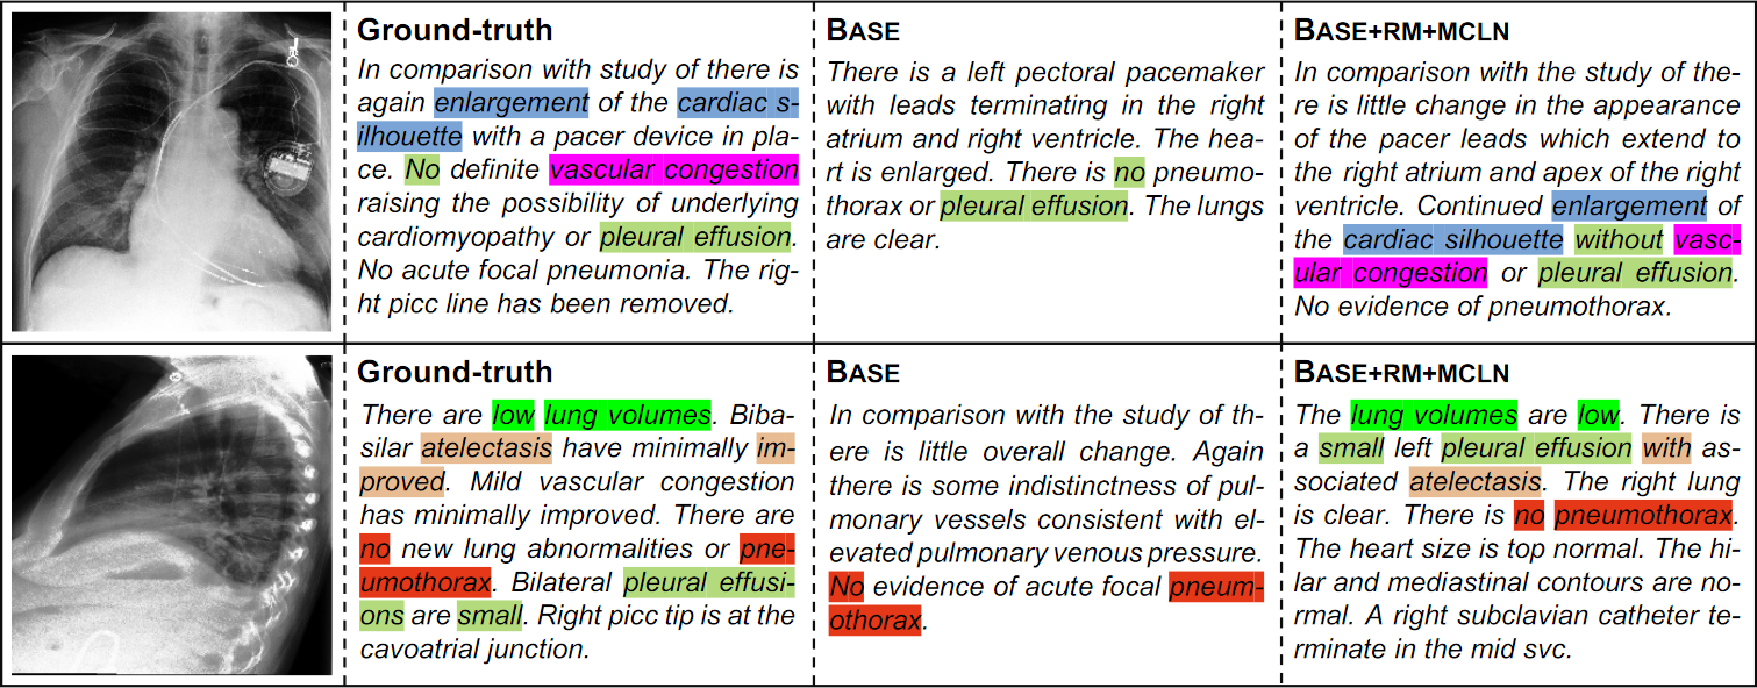
\includegraphics[width=145mm, height=57mm]{../img/ZhihongExample}
\caption{Examples of generated medical reports from \citet{chen2020generating}.}
\label{fig04:ZhihongExample}
\end{figure}

\citet{yuan2019automatic} paper proposes a hiearchical encoder-decoder architecture as we can see in the Figure \hyperref[fig05:YuanExample]{1.4} for the purpose of generating textual reports. Pairs of frontal and lateral X-ray images are used as an input to the network instead of single images, as the authors claim that the images should be complementary to each other instead of being processed independently. The RestNet-152 model pre-trained on the CheXpert\citep{irvin2019chexpert} dataset is utilized as the encoder with three outputs used later - the global and local features of the images, predticted observations and medical concepts. The decoder is hierarchical LSTM decoder comprising of the two parts: \textit{sentence decoder} and \textit{word decoder}. The sentence decoder takes visual features and generates hidden state for each sentence, which are along with the predicted medical concepts presented to the word decoder in order to generate the report. There are many other papers using a hierarchical architecture, e.g. \citet{huang2019multi}. \\

\begin{figure}[h]\centering
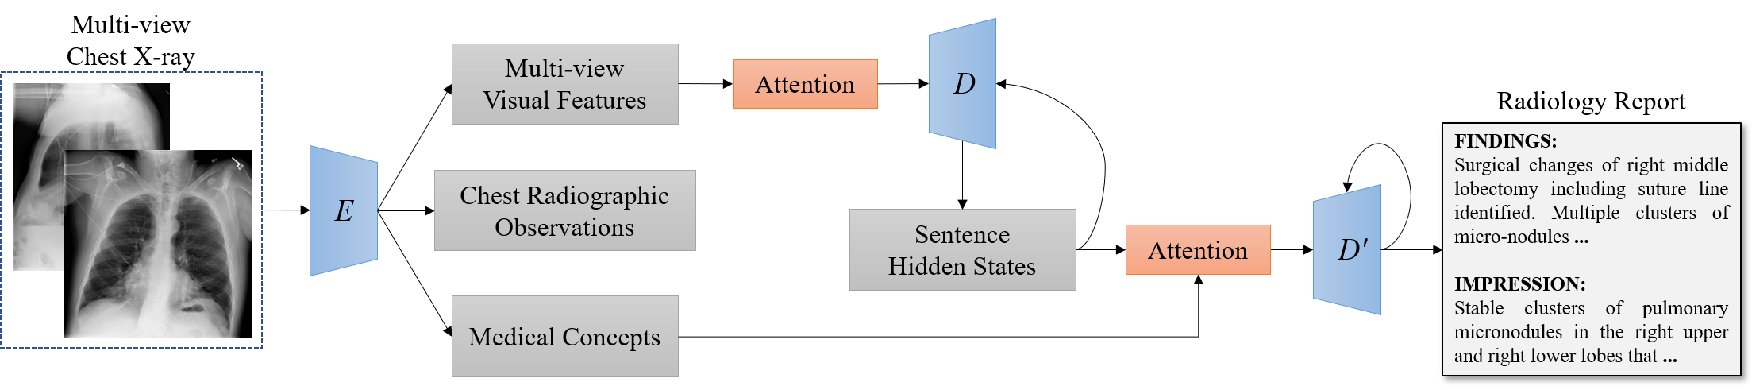
\includegraphics[width=145mm, height=32mm]{../img/YuanExample}
\caption{Hierarchical architecture from \citet{yuan2019automatic}.}
\label{fig05:YuanExample}

\textit{E} is encoder, \textit{D} is sentence decoder and \textit{D\textquotesingle} is word decoder.
\end{figure}

The last related project we mention in this work is CareBot\footnote[18]{\url{https://www.carebot.com/}}, which is being developed concurrently with our thesis. CareBot is a czech startup founded in 2021 as a reaction to the then ongoing Covid-19 pandemic. As in our work, CareBot focuses its attention mainly on the processing of chest X-rays using neural networks. However, unlike us it does not generate the textual reports for the doctors. Instead of textual reports, it focuses on finding and classifying a total of 15 different types of individual diseases on X-ray images and their subsequent spatial localization. Moreover, they already have a support from the medical environment.












\chapter{Title of the second chapter}

\section{Title of the first subchapter of the second chapter}

\section{Title of the second subchapter of the second chapter}


\chapter*{Conclusion}
\addcontentsline{toc}{chapter}{Conclusion}


%%% Bibliography
%%% Bibliography (literature used as a source)
%%%
%%% We employ bibTeX to construct the bibliography. It processes
%%% citations in the text (e.g., the \cite{...} macro) and looks up
%%% relevant entries in the bibliography.bib file.
%%%
%%% The \bibliographystyle command selects, which style will be used
%%% for references from the text. The argument in curly brackets is
%%% the name of the corresponding style file (*.bst). Both styles
%%% mentioned in this template are included in LaTeX distributions.

\bibliographystyle{plainnat}    %% Author (year)
% \bibliographystyle{unsrt}     %% [number]

\renewcommand{\bibname}{Bibliography}

%%% Generate the bibliography. Beware that if you cited no works,
%%% the empty list will be omitted completely.

\bibliography{bibliography}

%%% If case you prefer to write the bibliography manually (without bibTeX),
%%% you can use the following. Please follow the ISO 690 standard and
%%% citation conventions of your field of research.

% \begin{thebibliography}{99}
%
% \bibitem{lamport94}
%   {\sc Lamport,} Leslie.
%   \emph{\LaTeX: A Document Preparation System}.
%   2nd edition.
%   Massachusetts: Addison Wesley, 1994.
%   ISBN 0-201-52983-1.
%
% \end{thebibliography}


%%% Figures used in the thesis (consider if this is needed)
\listoffigures

%%% Tables used in the thesis (consider if this is needed)
%%% In mathematical theses, it could be better to move the list of tables to the beginning of the thesis.
\listoftables

%%% Abbreviations used in the thesis, if any, including their explanation
%%% In mathematical theses, it could be better to move the list of abbreviations to the beginning of the thesis.
\chapwithtoc{List of Abbreviations}

%%% Attachments to the master thesis, if any. Each attachment must be
%%% referred to at least once from the text of the thesis. Attachments
%%% are numbered.
%%%
%%% The printed version should preferably contain attachments, which can be
%%% read (additional tables and charts, supplementary text, examples of
%%% program output, etc.). The electronic version is more suited for attachments
%%% which will likely be used in an electronic form rather than read (program
%%% source code, data files, interactive charts, etc.). Electronic attachments
%%% should be uploaded to SIS and optionally also included in the thesis on a~CD/DVD.
%%% Allowed file formats are specified in provision of the rector no. 72/2017.
\appendix
\chapter{Attachments}

\section{First Attachment}

\openright
\end{document}
